\chapter{Reactor Characterization}
\label{Chapter:Modeling}
To design a reactivity controller for the \acl{msnb}, many components of the reactor needed to be characterized. The reactor was modeled in Serpent 2 to characterize the control drums using a series of criticality models. Depletion models were also used observe how the control drum characterization changes as the fuel is burned. Finally, a 1-dimension (spatial) uniform-state uniform-flow finite element model was developed in Python. This serves as the thermohydraulic process simulation needed to approximate the autonomous dynamic operation of the reactor during transients as well as study the performance improvement gained by application of the controller. 

\begin{figure}[!ht]
    \centering
    \resizebox{\textwidth}{!}{
\begin{tikzpicture}
    %Pre-filter
    \draw[->] (-6,0)node[anchor=east]{$\dot{Q}_{HEX}$} -- (-4.5,0);
    \draw (-4.5,-0.5) rectangle (-3.5,0.5) node[pos=0.5]{$F(s)$};
    %Sum
    \draw[->] (-3.5,0) -- (-2,0) node[pos=0.5,anchor=south]{$\dot{Q}_{Core}^{SP}$};
    \draw (-1.75,0) circle (0.25) node{\scriptsize$\textbf{-}$};
    %Controller
    \draw[->] (-1.5,0) -- (-0.5,0)node[pos=0.5,anchor=south]{$e$};
    \draw (-0.5,-0.5) rectangle (0.5,0.5) node[pos=0.5]{$C(s)$};
    \draw[->] (0.5,0) -- (1.5,0) node[pos=0.5,anchor=south]{$u_{CD}$};
    %Actuator
    \draw (1.5,-0.5) rectangle (2.5,0.5) node[pos=0.5]{$A(s)$};
    \draw[->] (2.5,0) -- (3.5,0) node[pos=0.5,anchor=south]{$\rho_{CD}$};
    %Sum
    \draw (3.75,0) circle (0.25) node{\scriptsize$\textbf{+}$};
    %Process
    \draw[->] (4,0) -- (5,0) node[pos=0.5,anchor=south]{$\rho$};
    \draw (5,-0.5) rectangle (6,0.5) node[pos=0.5]{$P(s)$};
    \draw[->] (6,0) -- (8,0) node[anchor=west]{$\dot{Q}_{Core}$};
    %Transducer
    \draw[->] (7,0) -- (7,-1.5) -- (2.5,-1.5);
    \draw (1.5,-2) rectangle (2.5,-1) node[pos=0.5]{$H(s)$} ;
    \draw[->] (1.5,-1.5) -- (-1.75,-1.5) -- (-1.75,-0.25);
    %Passive Feedback
    %Core Feedback
    \draw[->] (7,0) -- (7,2.5);
    \draw (6.5,2.5) rectangle (7.5,3.5) node[pos=0.5]{$G_{C}(s)$};
    \draw[->] (6.5,3) -- (4.25,3);
    %HEX Feedback
    \draw[->] (-5,0) -- (-5,2.5);
    \draw (-4.5,2.5) rectangle (-5.5,3.5) node[pos=0.5]{$G_{H}(s)$};
    \draw[->] (-4.5,3) -- (3.25,3)node[pos=0.5,anchor=south]{$T_{cold}$};
    %Sum
    \draw (3.75,1.5) circle (0.25) node{\scriptsize$\textbf{+}$};
    \draw[->](3.75,1.25) -- (3.75,0.25);
    %TemperatureFeedback
    \draw (1.5,1) rectangle (2.5,2) node[pos=0.5]{$\alpha_T$};
    \draw[->] (2.5,1.5) -- (3.5,1.5) node[pos=0.5,anchor=south]{$\rho_{T}$};
    %FlowFeedback
    \draw (3.25,2.5) rectangle (4.25,3.5) node[pos=0.5]{$\alpha_F$};
    \draw[->] (3.75,2.5) -- (3.75,1.75) node[pos=0.5,anchor=west]{$\rho_{F}$};
    %Downcomer
    \draw[->] (0,3) -- (0,2);
    \draw (-0.5,1) rectangle (0.5,2) node[pos=0.5]{$\theta_{DC}$};
    \draw[->] (0.5,1.5) -- (1.5,1.5);
    %Riser
    \draw[->] (5.375,3) -- (5.375,4.5) -- (0.5,4.5) node[pos=0.5,anchor=south]{$T_{hot}$};
    \draw (-0.5,4) rectangle (0.5,5) node[pos=0.5]{$\theta_{R}$};
    \draw[->] (-0.5,4.5) -- (-5,4.5) -- (-5,3.5);


\end{tikzpicture}
}
    \caption[Control loop of a natural circulation \acs{msnb}]{Control loop of a natural circulation \acs{msnb}. It is a normal feedback loop with a pre-filter, with the addition of the passive feedback mechanisms. The core ($\dot{Q}_{Core}$) and heat exchanger ($\dot{Q}_{HEX}$) powers go through the respective temperature dynamics ($G_C$ and $G_H$) and time delays for the riser ($\theta_R$) and downcomer ($\theta_{DC}$) before being converted to reactivity by the temperature($\alpha_T$) and flow ($\alpha_F$) feedback mechanisms. The passive reactivity feedback is combined with the control drum reactivity ($\rho_{CD}$) and fed into the reactor dynamics ($P(s)$).  }
    \label{fig:ReactorControlLoop}
\end{figure}

\section{Reactor Design}\label{Section:Design}
The \acs{msnb} is self contained in a 145 cm diameter, 242 cm tall cylindrical rector vessel that is buried in the ground or concrete for shielding purposes. The core is a concentric 166 cm tall cylinder 50 cm in diameter surrounded by a large reflector into which 8 equally spaced control drums are embedded. A neutron trap sits above the reflector to separate the riser, where fission caused by delayed neutrons occurs at a significant rate, from the heat exchanger. The downcomer is an annular gap between the outer part of the reflector and the outer reactor vessel. It has flow area identical to the core, and returns cold salt from the outlet of the heat exchanger to the inlet plenum.

Figure \ref{fig:Plotter-YZ} is an axial cross-section of the \acs{msnb}. Figure \ref{fig:Plotter-XY} contains four radial cross-sections of the \acs{msnb}. These two figures were generated by the Serpent model described in Section \ref{Section:Serpent}. In these models, \UF dissolved in \flinak is depicted as varying shades of red depending on temperature, beryllium-oxide is light-blue, boron-carbide is green, graphite is yellow, stainless steel is light-gray, Hastelloy-N is medium-gray, barite concrete is dark-gray, and air is pink. The reactor is buried in barite concrete for radiation shielding purposes, and the top is at the surface so secondary coolant systems can readily be connected.

\begin{figure}[ht!]
    \centering
    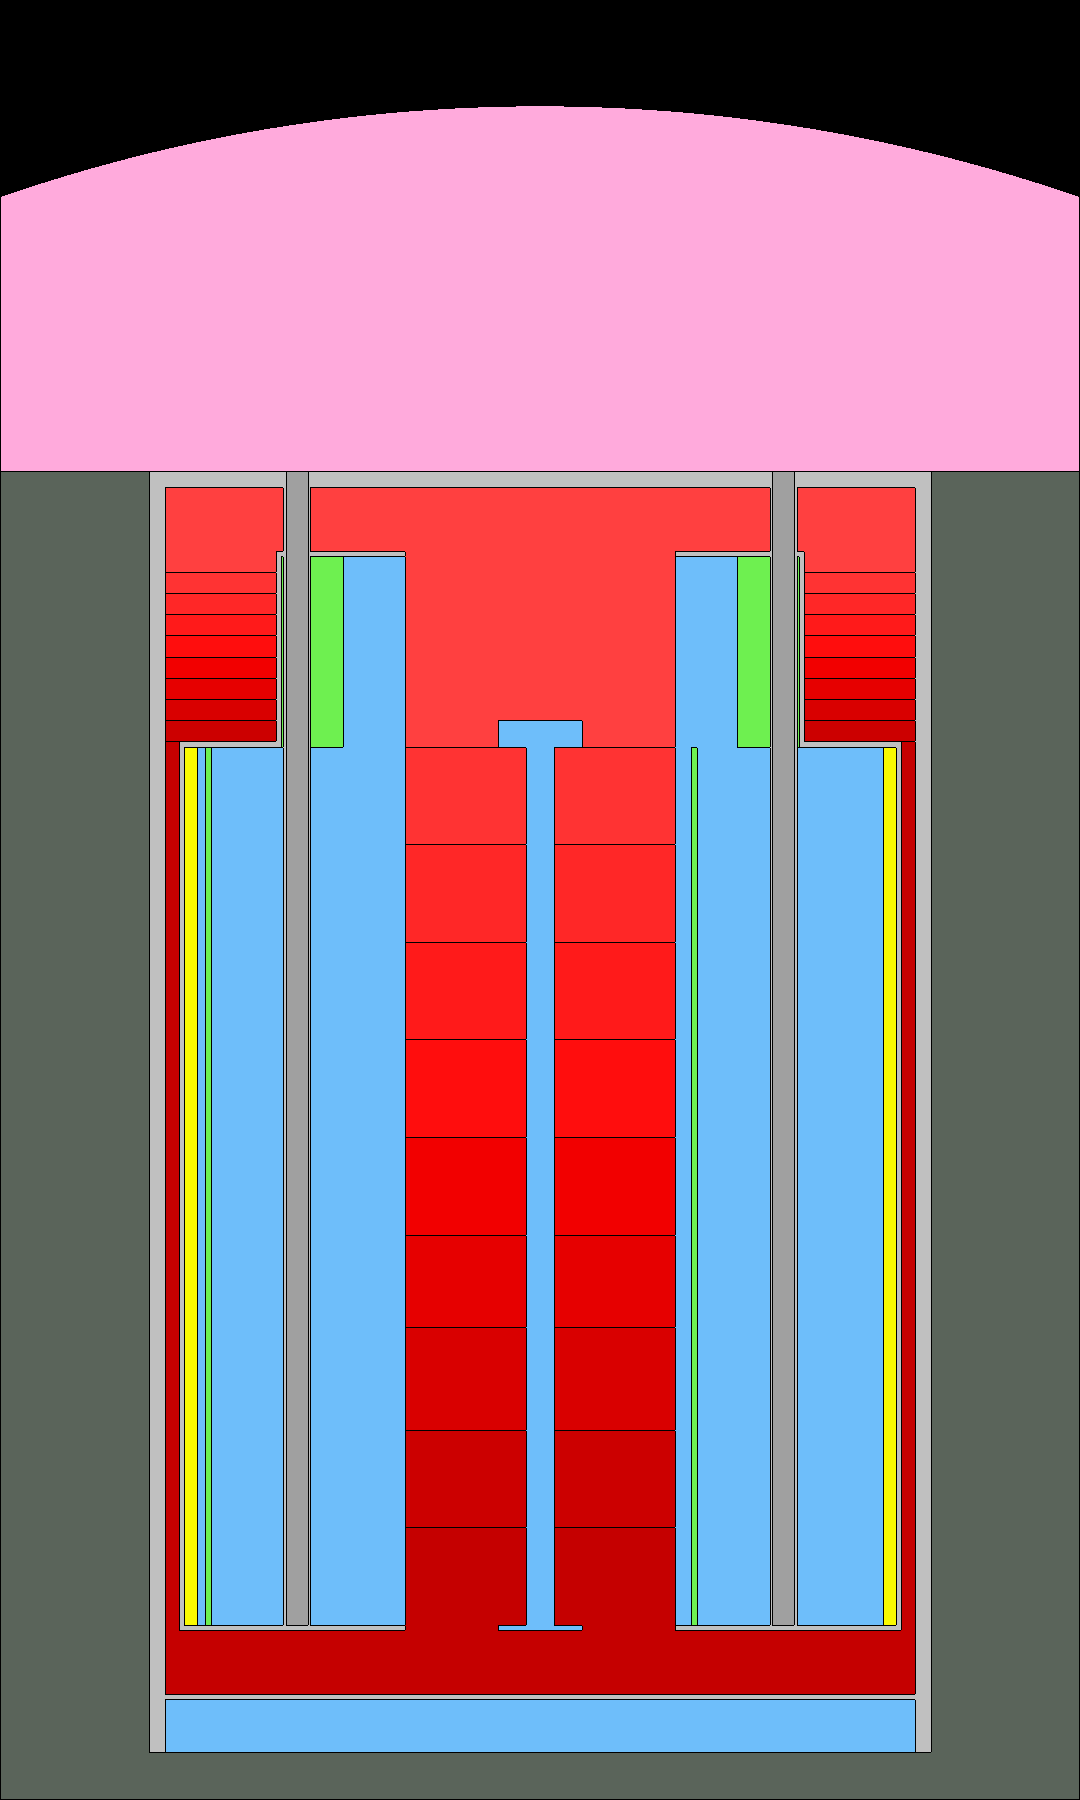
\includegraphics[width=0.75\textwidth]{Plotter/0.0/MSNB_geom1.png}
    \caption[Y-Z view of \acs{msnb}]{Y-Z view of \acs{msnb}. Molten salt is shown in red, with darker shades corresponding to a lower temperature and higher density. The core is surrounded by the beryllium-oxide reflector (blue) and the boron-carbide absorber plate (green). The core is separated from the riser by a a perforated reflector plate and the riser is separated from the heat exchanger by an absorbing ring. From this angle the internal moderating structure appears as only the center rod, as the fins exist in other planes.}
    \label{fig:Plotter-YZ}
\end{figure}
\clearpage
\begin{figure}[!ht]
    \centering
    \subfloat[\centering Inlet Plenum]{
\includegraphics[width=0.49\textwidth]{Plotter/0.0/MSNB_geom2}}
    \subfloat[\centering Core]{\includegraphics[width=0.49\textwidth]{Plotter/0.0/MSNB_geom4}}
    \quad
    \subfloat[\centering Heat Exchanger]{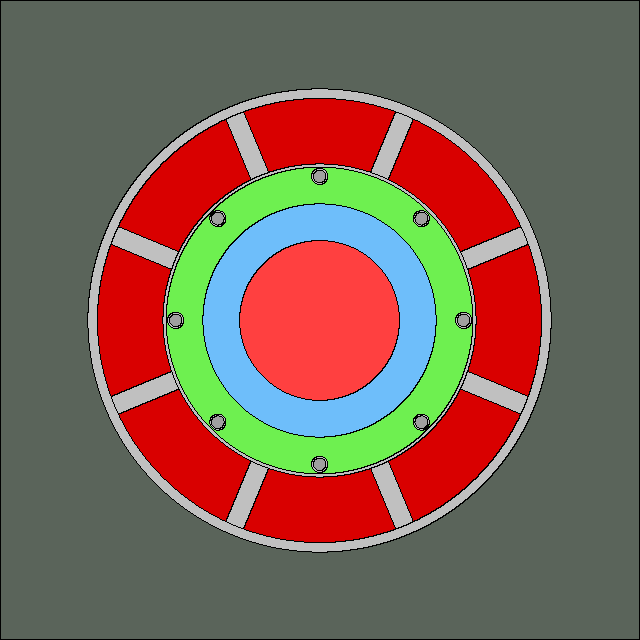
\includegraphics[width=0.49\textwidth]{Plotter/0.0/MSNB_geom6}}
    \subfloat[\centering Spoke]{
\includegraphics[width=0.49\textwidth]{Plotter/0.0/MSNB_geom8}}
    \caption[X-Y Views of \acs{msnb}]{X-Y Views of \acs{msnb}
    \begin{enumerate*}[label=\alph*)]
        \item Molten salt from the downcomer travels inward below the reflector the center, where it rises to enter the core;
        \item The core is surrounded by the reflector and control drums, which may be adjusted to manipulate criticality. The reflector and downcomer are separated by a graphite shield;
        \item The molten salt in the outer ring is in the heat exchanger. As it sinks, heat is being rejected to the secondary coolant (not modeled). A ring of boron-carbide ensures that delayed neutrons emitted in the riser do not transport to the heat exchanger; 
        \item Molten salt exiting the riser travels radially outward to the top of the heat exchanger;
    \end{enumerate*}}
    \label{fig:Plotter-XY}
\end{figure}

\subsection{Molten Salt}
The molten salt in the \acs{msnb} serves as both the primary coolant and the fuel. It is composed of 18 mol\% \acs{haleu} \UF \; (enriched to 19.75\%) dissolved in eutectic \flinak (enriched to 99.99\% \Li[7]). It is composed of about 1.4 atom\% \U[235]. The remaining composition is listed in Table \ref{tab:saltcomp}. This molten salt fuel system has been studied in previous work \cite{CarterPHD}. The present work leverages intermediate calculations, such as the thermophysical property temperature functions - density\footnote{note the use of $\varrho$ to distinguish density from reactivity ($\rho$)} ($\varrho$) and heat capacity ($c_p$) - of the salt:

\begin{equation}\label{eq:saltdens}
    \varrho[kg/m^3] = 4682.0365 - 0.94301046\cdot T[K] 
\end{equation}
\begin{equation}\label{eq:saltcp}
    c_p[kJ/kg-K] = 0.97678 + 0.0010634\cdot T[K]
\end{equation}

\flinak was selected for study due to its thermal properties and prevalence in \acs{msr} research, and \UF \; was selected as it is soluble in \flinak to a concentration that has a wide liquidus range, supports criticality in the reactor geometry necessary to fit into a shipping container, and provides adequate power density for thermal hydraulic design. 

\begin{table}[ht!]
    \caption[Molten salt composition]{\raggedright Composition of molten salt prior to burn-up}
    \centering
    \begin{tabular}{rl|cc}
     Element&Isotope&Atom Percent & Weight Percent \\ \hline
     Fluorine  & 19  & 60.63 \%  & 32.40 \% \\  \hline
     Lithium   & 6   & 15 ppm    & 2.5 ppm  \\
               & 7   & 15.01 \%  & 2.96 \%  \\ \hline
     Sodium    & 23  &  3.71 \%  & 2.40 \%  \\ \hline
     Potassium & 39  & 12.61 \%  & 13.82 \% \\
               & 41  & 0.95 \%  & 1.09 \%  \\ \hline
    Uranium    & 235 & 1.40 \%   & 9.25 \%  \\
               & 238 & 5.69 \%   & 38.08 \% \\
    \end{tabular}
    \label{tab:saltcomp}
\end{table}

\subsection{Control Drums}
Control drums are cylinders of neutron reflector with a portion of the circumference replaced with a neutron absorber. As is depicted by Figure \ref{fig:Plotter-CD}, rotating the control material inward inhibits the neutron chain reaction. This concept is used in the Advanced Test Reactor at \acs{inl}, using a beryllium/hafnium design \cite{atr}. It is also a popular concept for accident tolerance in space reactors, which have the potential to crash during launch \cite{AT-CD}. 

\begin{figure}[!ht]
    \centering
    \subfloat[\centering Least Reactive]{\includegraphics[width=0.33\textwidth]{Plotter/0.0/MSNB_geom4}}
    \subfloat[\centering Initial Criticality]{\includegraphics[width=0.33\textwidth]{Plotter/112.0/MSNB_geom4}}
    \subfloat[\centering Most Reactive]{\includegraphics[width=0.33\textwidth]{Plotter/180.0/MSNB_geom4}}
    \caption[X-Y View of \acs{msnb} - Control Drums]{X-Y Views of \acs{msnb} with control drums in three orientations:
    \begin{enumerate*}[label=\alph*)]
        \item 0 degrees, which is used to test the reactor's shutdown margin;
        \item 112 degrees, which is the initial critical orientation; and 
        \item 180 degrees, which is used to test the reactor's excess reactivity; 
    \end{enumerate*}
    Beryllium oxide is depicted in blue while boron carbide is green.}
    \label{fig:Plotter-CD}
\end{figure}

Each of the eight drums in the \acs{msnb} is the same height as the core, 17 cm in radius, and has a 1 cm thick absorber pad covering 25\% of the circumference. This study uses beryllium oxide as the reflector material for cost, machinability, and radiation damage considerations, and boron carbide for the absorber, as it provides adequate shutdown margin while preserving more excess reactivity than hafnium. 

In addition to the higher absorption cross-section, hafnium also is considered a non-burnable poison, as the transmutation products also have a high cross-section. In contrast, the products of \B[10] capture are essentially transparent to neutrons. It was confirmed using a burn-up study that the boron carbide would not be significantly depleted during the life of the \acs{msnb}.

\subsection{In-Pile Moderator}
Previous work has suggested an in-pile helix made of a neutron scattering material to extend the in core flow path and simultaneously soften the neutron energy spectrum to provide more excess reactivity \cite{CarterPHD}. This work investigates a simpler version of this concept focused only on providing excess reactivity. It is composed of 8 radial fins spaced 45 degrees apart, and is made from beryllium oxide.

\subsection{Structural Materials}
The reactor vessel, along with supplementary structural materials such as reflector and moderator supports, heat exchangers, and control drum driveshaft sheaths are made from 316 stainless steel. Control drum driveshafts are made from Hastelloy-N, a nickel-chromium-molybdenum alloy that is resistant to corrosion from high temperature fluoride salts. The reactor vessel is encased in barite concrete for added radiation shielding.

\section{Neutronics Modeling}\label{Section:Serpent}
The reactor described in Section \ref{Section:Design} was modeled in Serpent 2, making use of the Sawtooth supercomputer at \acs{inl}'s \acs{hpc} center. The fuel was stratified for an expected temperature rise using \ref{eq:saltdens} and redundant material cards. A python script was written to automatically generate the input cards that reflect a specific molten salt composition and control drum angle\footnote{The input file writing script is available at \href{https://github.com/sjroot97/MSNB-Serpent2-Autodeck}{https://github.com/sjroot97/MSNB-Serpent2-Autodeck} and is also included in Appendix \ref{app:Serpent}.} This made it easy to submit batches of several criticality models sequentially to Sawtooth using a Bash submission script.

 An alternating methodology of criticality and burn-up models was employed to characterize the control drums. First, the $k_{eff}$ for the entire range of control drum angles (from 0 to 180 degrees) was obtained using a criticality model that used 1,000,000 source particles per cycle, 500 active cycles, and 100 inactive cycles. With 32 nodes parallelizing 4 threads, each control drum angle took between 2 and 5 minutes to complete. This allowed the entire range of control drum angles to be simulated with a wall-time of 2 hours.  

 With the entire control drum angle vs. reactivity curve defined, the unity point was calculated and a burn-up model was conducted at that angle. A stochastic volume calculation was obtained using the `mcvol' subroutine, and the depletion module was loaded at 10 MW with a time-step of 6 hours until \Xe reached equilibrium, and 6 months following. Originally, smaller time-steps of 1-5 days were used to study the change to the control drum-reactivity curve as \Sm built up. This was forgone after finding that \Sm acts as a non-equilibrium fission product neutron poison at the relatively low power density studied. 
 
 To approximate the flowing and electrolytic nature of the \acs{msnb} that disperses fission products over time, the burn-up studies were completed without fuel stratification. This is in contrast to how solid fueled burn-up studies are often conducted, where depletion zones are employed to resolve the effects of the spatial neutron flux profile. This provided the new molten salt and boron carbide compositions for the next set of criticality models.

\section{Process Simulation}\label{Section:Python}
A multiphysics transient simulation was written in Python to study the \acs{msnb} in dynamic operations by the coupling of thermal hydraulics and neutronics. First principle physics were implemented to approximate the expected behavior of the reactor. It is not meant to be a digital twin, but rather a responsive tool for the design of the power controller\footnote{The input file writing script is available at \href{https://github.com/sjroot97/MsNB-Simulator/}{https://github.com/sjroot97/MsNB-Simulator/} and is also included in Appendix \ref{app:Simulator}.}.

The simulation is built on three physics principles: 
\begin{enumerate*}
    \item Thermally driven natural circulation flow mode, where the pressure differential driven by a difference in density between the hot and cold leg is equilibrated by frictional losses to calculate the flow rate;
    \item Reactor point kinetics, where the compound passive dynamics are used to time-advance the reactor power based; and
    \item Uniform-state uniform-flow time and spatial advancement of energy in the flow loop.;
\end{enumerate*}

\begin{figure}[ht!]
    \centering
    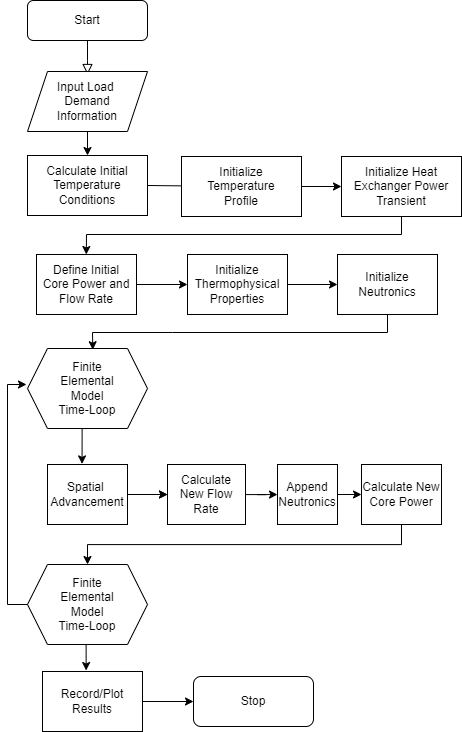
\includegraphics[width=0.5\textwidth]{FlowDiagram}
    \caption[Process simulator logic flow diagram]{\raggedright Logic flow diagram for the \acs{msnb} transient process simulator.}
    \label{fig:PythonFlowDiagram}
\end{figure}

Figure \ref{fig:PythonFlowDiagram} is a logic flow diagram that describes how the code simulates the dynamic operation of the \acs{msnb}. Similar to previous work, the flow loop of the reactor was simplified into a 1-dimensional flow loop with equal flow area throughout \cite{CarterNumerical,CarterPHD,Root}. The simulator is broken up into two different sections - first the problem is set-up, then the transient is simulated in a finite element time loop with time steps of 1 second. The model is described in Sections \ref{Section:initial} and \ref{Section:advance}, and rely on the parameters listed in Table \ref{tab:FEMparams}

\begin{table}[ht!]
    \caption[\acs{msnb} simulation parameters]{\raggedright System parameters used in the simulation of the \acs{msnb} \cite{CarterNumerical}. }
    \centering\begin{tabular}{r|ccl}
        &  Value &  Unit &  Description \\ \hline
    $\alpha_T$ & $-3.5$ & pcm/K & Temperature reactivity feedback coefficient \\
    $\ell^*$ & $1.63 \times 10^{-4}$  & sec & Mean neutron generation time \\
    $\beta_{eff}$ & $6.96 \times 10^{-3}$  & - & Effective delayed neutron fraction \\
    $\lambda$ & $0.1$  & sec$^{-1}$ & One-group delayed neutron precursor decay constant \\
    $\xi$ & $25$  & - & Pressure loss coefficient \\
    $h$ & $1.09$  & m & Height between thermal centers \\
    $\alpha_f$ & $-0.3398$ & s/cm & Flow reactivity feedback coefficient \\
    $A_x$ & $0.4$  & m$^{2}$ & Cross-sectional flow area \\
    $g$ & $9.81$  & m/s$^{2}$ & Acceleration due to gravity \\
    $\delta t$ & $1$  & sec & Time-step duration  \\
    $\delta x$ & $1$  & mm & Control volume length  \\
    \end{tabular}
    \label{tab:FEMparams}
\end{table}

\subsection{Model Initialization}\label{Section:initial}
The code first takes inputs to define the heat exchanger power transient that is to be studied. The reactor is initially assumed to be steady-state and critical, so the temperature is constant in the chimney and downcomer, and heating/cooling are uniform and equal in the core and heat exchanger. A binary search algorithm is used to iteratively find the cold leg ($T_{cold}$) temperature that corresponds to the initial power requirement with a hot leg temperature ($T_{hot}$) of 700 $^o$C. The heat exchanger power ($\dot{Q}_{HEX}$) is calculated by:

\begin{equation}
    \dot{Q}_{HEX} = \bar{\varrho}_{HEX} A_x v \bar{c_p}_{HEX} (T_{hot} - T_{cold})
\end{equation}

Where $\bar{\varrho}_{HEX}$ and $\bar{c_p}_{HEX}$ are the average density and heat capacity in the heat exchanger, $A_x$ is the cross-sectional flow area within the reactor, and $v$ is the velocity of the salt in the loop. The key assumption for this model is that the flow velocity during a given time-step is uniform throughout the flow loop, both during steady-state and unsteady-state time periods. This assumption allows for a simple spatial advancement, and an explicit total energy balance solution, which is described in detail in Section \ref{Section:advance}. The flow velocity is calculated based on the temperature profile, assuming a natural circulation flow mode:

\begin{equation}\label{eq:saltvelo}
    v = \sqrt{\nicefrac{2gh(\varrho_{cold}-\varrho_{hot})}{\xi\varrho}}
\end{equation}

where $g$ is the gravitational acceleration, $h$ is the height between thermal centers, $\xi$ is the pressure loss coefficient (estimated to be 25.0 by STAR-CCM+ \cite{CarterNumerical}), $\bar{\varrho}_{cold}$ and $\bar{\varrho}_{hot}$ are the average salt densities of the cold and hot leg, and $\bar{\varrho}$ is the average salt density of the entire reactor loop.

The criticality assumption must be satisfied between the two passive feedback mechanisms. Flow reactivity ($\rho_f$) is calculated explicitly, while temperature reactivity ($\rho_T$) is calculated relatively \cite{Kerlin}:

\begin{equation}\label{eq:flowreac}
    \rho_f = -\frac{L}{L+H}\beta_{eff}\left(1-e^{-v\alpha_f}  \right)
\end{equation}
\begin{equation}
    \Delta\rho_T = \alpha_T\Delta T
\end{equation}

where L and H are the out-of-core and in-core lengths, $\beta_{eff}$ is the effective delayed neutron fraction, and $\alpha_f$ and $\alpha_T$ are the flow reactivity feedback coefficient and temperature reactivity feedback coefficient. Table \ref{tab:flowloop} contains the loop coordinates for key points in the \acs{msnb} \cite{CarterNumerical}. 

\begin{table}[ht!]
    \caption[\acs{msnb} loop coordinates]{\raggedright \acs{msnb} loop coordinates for the transitions between equipment \cite{CarterNumerical}. }
    \centering\begin{tabular}{ll}
        Location in Reactor & Loop Coordinate (mm)\\\hline
        Core Inlet & 0, 5710 \\
        Core Outlet & 1660 \\
        Top of Hot Leg & 2090 \\
        Heat Exchanger Inlet & 2340 \\
        Heat Exchanger outlet & 2825 \\
        Bottom of Cold Leg & 4975 \\        
    \end{tabular}
    \label{tab:flowloop}
\end{table}

For a critical core, the initial temperature reactivity is defined as equal and opposite the initial flow reactivity. This is satisfied by orienting the control drums at their bias point, such that control reactivity ($\rho_C$) is null.

\subsection{Discrete Time Step}\label{Section:advance}
The process simulator uses two steps to simulate the passage of time:
\begin{enumerate*}
    \item The flow loop is advanced by the distance the molten salt travels during the discrete time step; and 
    \item Time dependent parameters are updated.
\end{enumerate*}

\subsubsection{Spatial Advancement of Flow Loop}
The spatial advancement of the flow loop is a 1D+time computational fluid dynamics problem, with each millimeter long slice ($\delta x$) of the entire cross-section of the flow loop being treated as a control volume. With the assumption of uniform flow velocity around the loop for each discrete time step, the continuity equation for the system can be expressed as:

\begin{equation}
    \delta x A_x \frac{d\varrho}{dt} = v A_x(\varrho_{in}-\varrho_{out})
\end{equation}

In solving the total energy balance for the time-step, it is useful to convert the temperature profile ($T_x$) to an energy profile ($mu_x$). This is done by using the temperature functions for density, \ref{eq:saltdens}  and heat capacity, \ref{eq:saltcp} and assuming a reference temperature ($T_r$) where the energy is defined as null:

\begin{equation}\label{eq:T2mu}
    mu_x = \varrho(T_x)\delta x A_x
             c_p\left(\nicefrac{T_x+T_r}{2}\right)(T_x-T_r) 
\end{equation}

By neglecting gravimetric, kinetic, and pressure-volume differentials, and assuming the uniform-state uniform-flow condition, where the thermophysical and thermodynamic properties of the control volume are considered equal throughout, the discrete total energy balance for each control volume becomes:

\begin{equation}
    \frac{d(mu)}{dt} = mu_{enter} - mu_{exit} + Q_{c.v.}
\end{equation}

In the simulator, the energy profile is stored as a numpy array, with the energy in each control volume being stored as a single element in the ordered series. During a discrete time-step, the salt described by the element corresponding to the control volume exits the control volume, the element lagging by $v\delta t$ enters the control volume, and every element in-between both enters and exits the control volume. As such, each of these interior elements can be neglected. $mu_x$ does not need to be modified to obtain $mu_{exit}$, and $mu_{enter}$ can be obtained by using the numpy `roll' method, passing a value of $v\delta t$ for the `shift' argument. The outlets the heat exchanger and core must be flattened to account for edge heating/cooling effects. 

The control volume power  ($Q_{c.v.}$) is calculated ay assuming uniform heating/cooling and preserving the convention of negative heat rejection:

\begin{equation}
    Q_{c.v.} = \left\{ 
        \begin{matrix*}[l]
            \nicefrac{Q_{Core}}{l_{core}} &\;,\; Core\\
            \;\;\;0                       &\;,\; Riser\\
            \nicefrac{-Q_{HEX}}{l_{HEX}}  &\;,\; Heat Exchanger\\
            \;\;\;0                       &\;,\; Downcomer
        \end{matrix*}
    \right.
\end{equation}

After the discrete time-step, the new energy profile is calculated using Euler's forward method:

\begin{equation}
    mu[t+\delta t] = mu[t] + \delta t\frac{d(mu)}{dt}[t]
\end{equation}

Then, the updated temperature profile can be obtained from the updated energy profile by inverting \ref{eq:T2mu}. This is not a readily separable function, so an expected range of temperatures was put through the forward function, and the results were fit to a 6th order polynomial to define an inverse function. With the updated temperature profile, the rest of the time variables can be updated to solve for the new core power.

\subsubsection{Updating Time Variables}
First, the updated temperature profile is used to calculate the new molten salt flow velocity using \ref{eq:saltvelo}, which is in turn used to calculate the new flow reactivity using \ref{eq:flowreac}. Then the change in average core temperature is used to calculate the new temperature reactivity:

\begin{equation}
    \rho_T[t+\delta t] = \rho_T[t] + \alpha_T\Delta T_{core}
\end{equation}

Each reactivity phenomenon is summed, and reactor period ($\tau$) is obtained using one group reactor point kinetics:

\begin{equation}
    \tau = \frac{\ell^{*}}{\rho}
         +\frac{\beta_{eff}-\rho}{\lambda\rho + \dot{\rho}}
\end{equation}

where $\lambda$ is the delayed neutron precursor decay constant and $\dot{\rho}$ is the reactivity rate of change \cite[Ch. 6]{DH}. Finally, the updated power can be obtained from the e-folding equation:

\begin{equation}
    Q_{core}[t+\delta t] = Q_{core}[t] e^{\nicefrac{\delta t}{\tau}}
\end{equation}

With the new power, the entire sequence of calculations can be repeated for the next discrete time-step, repeating until the simulation is over. These steps result in a first principles based multiphysics model that simulates compound passive feedbacks to compute the approximate behavior of a natural circulation \acs{msnb} during dynamic operation.